\documentclass[journal,twoside,web]{ieeecolor}
\usepackage{generic}
\usepackage{cite}
\usepackage{amsmath,amssymb,amsfonts}
\usepackage{algorithm}
\usepackage{algorithmic}
\usepackage{graphicx}
\usepackage{textcomp}
\makeatletter
\def\BState{\State\hskip-\ALG@thistlm}
\makeatother

\def\BibTeX{{\rm B\kern-.05em{\sc i\kern-.025em b}\kern-.08em
    T\kern-.1667em\lower.7ex\hbox{E}\kern-.125emX}}
\markboth{\journalname, Project IMP, 12/11/2017}
{FANG Yidong, An Evolutionary Algorithm with Local Search for the Capacitated Arc Routing Problem}
\begin{document}
\title{An Implementation of Efficient Influence Maximization Algorithm in Social Networks}
\author{FANG Yidong, Student No.11510493 \IEEEmembership{CSE, Southern University of Science and Technology}
}

\maketitle

\begin{abstract}
Influence maximization is the problem of finding a small subset of nodes (seed nodes) in a social network that could maximize the spread of influence. In this paper, we study the efficient influence maximization from two complementary directions. One is to improve the original greedy algorithm of \cite{Kempe2003} and its improvement \cite{Leskovec2007} to further reduce its running time, and the second is to propose new degree discount heuristics that improves influence spread. In this project, we implemented our algorithm based on the algorithm metion in \cite{Chen2009} based on Python2.
\end{abstract}

\begin{IEEEkeywords}
Influence Maximization;
greedy algorithm;
heuristic algorithm;
social network;
discounted degree algorithm;

\end{IEEEkeywords}

\section{Introduction}
\label{sec:introduction}
\IEEEPARstart{R}{cently} many large-scale online social network sites, such as Facebook and Friendster, become successful because they are very effective tools in connecting people and bringing small and disconnected offline social networks together. Moreover, they are also becoming a huge dissemination and marketing platform, allowing information and ideas to influence a large population in a short period of time. However, to fully utilize these social networks as marketing and information dissemination platforms, many challenges have to be met. In this paper, we present our work towards addressing one of the challenges, namely finding influential individuals
efficiently in a large-scale social network. \par
Consider the following hypothetical scenario as a motivating example. A small company develops a cool online application for an online social network and wants to market it through the same network. It has a limited budget such that it can only select a small number of initial users in the network to use it (by giving them gifts or payments). The company wishes that these initial users would love the application and start influencing their friends on the social network to use it, and their friends would influence their friends’ friends and so on, and thus through the word-of-mouth effect a
large population in the social network would adopt the application. The problem is whom to select as the initial users so that they eventually influence the largest number of people in the network, i.e., the problem of finding influential individuals in a social network. \par
This problem, referred to as influence maximization, would be of interest to many companies as well as individuals that want to promote their products, services, and innovative ideas through the powerful word-of-mouth effect (or called viral marketing). Online social networks provide good opportunities to address this problem, because they are connecting a huge number of people and they collect a huge amount of information about the social network structures and communication dynamics. However, they also
present challenges to solve the problem. The social networks are large-scale, have complex connection structures, and are also very dynamic, which means that the solution to the problem needs to be very efficient and scalable. \par
Domingos and Richardson \cite{Domingos2001} are the first to study influence maximization as an algorithmic problem. Their methods are probabilistic, however. Kempe, Kleinberg, and Tardos \cite{Kempe2003} are the first to formulate the problem as the following discrete optimization problem. A social network is modeled as a graph with vertices rep-
resenting individuals and edges representing connections or relationship between two individuals. Influence are propagated in the network according to a stochastic cascade model. Three cascade models, namely the independent cascade model, the weight cascade model, and the linear threshold model, are considered in \cite{Kempe2003}. Given a social network graph, a specific influence cascade model,and a small number k, the influence maximization problem is to find k vertices in the graph (refered to as seeds) such that under the influence cascade model, the expected number of vertices influenced by the k seeds (referred to as the influence spread in the paper) is the largest possible.\par
Kempeet al.provethat theoptimizationproblemis NP-hard, and present a greedy approximation algorithm applicable to all three models, which guarantees that the influence spread is within $(1- 1/e)$ of the optimal influence spread. They also show through experiments that their greedy algorithm significantly outperforms the
classic degree and centrality-based heuristics in influence spread. However, their algorithm has a serious drawback, which is its efficiency. A key element of their greedy algorithm is to compute the influence spread given a seed set, which turns out to be a difficult task. Instead of finding an exact algorithm, they run Monte-Carlo
simulations of the influence cascade model for sufficiently many times to obtain an accurate estimate of the influence spread. As a result, even finding a small seed set in a moderately large network (e.g. 15000 vertices) could take days to complete on a modern server machine.\par
Several recent studies aimed at addressing this efficiency issue. In \cite{Kimura2006}, Kimura and Saito propose shortest-path based influence cascade models and provide efficient algorithms of compute influence spread under these models. However, since the influence cascade models are different, they do not directly address the efficiency issue of the greedy algorithms for the cascade models studied in \cite{Kempe2003}. \par
In \cite{Leskovec2007}, Leskovec et al. present an optimization in selecting new seeds, which is referred to as the “Cost-Effective Lazy Forward” (CELF) scheme. The CELF optimization uses the submodular-
ity property of the influence maximization objective to greatly reduce the number of evaluations on the influence spread of vertices. Their experimental results demonstrate that CELF optimization could achieve as much as 700 times speedup in selecting seed
vertices, which is a very impressive result. However, our experiments show that the improved algorithm still takes a few hours to complete in a graph with a few tens of thousands of vertices, so it is still not efficient for large-scale networks.\par
In this project, we mainly followed the idea from Wei Chen \cite{Chen2009}, and we implemented two kinds of algorithm to solve the problem. One algorithm is an improved algorithm with a combination of improved Monte-Carlo evaluation of the spread and CELF, the other algorithm is heuristic algorihtm called discounted degree algorith. According to the paper, the improved algorithm algorithm outperforms almost all the other algorithm w.r.t the resulting spread. And also, with a significant effciency (with 10 seconds for graph with 10,000 vertices), the heristic algorithm gives an acceptable spread and better than other heristic algorithms.

\section{Improved Greedy Algorithm}
In this section, we discuss improvement of the greedy algorithm proposed by Kempe, et al. \cite{Kempe2003} for the independent cascade model as well as the weighted cascade model.

\subsection{Problem definition and the greedy algorithm}
A social network is modeled as an undirected graph $G = (V,E)$, with vertices in $V$ modeling the individuals in the network and edges in $E$ modeling the relationship between individuals. \par
Let S be the subset of vertices selected to initiate the influence propagation, which we call the seed set. Let $RanCas(S)$ denote the random process of influence cascade from the seed set $S$, of which the output is a random set of vertices influenced by $S$. Algorithms in this project take the graph $G$ and a number $k$ as input and generate a seed set $S$ of cardinality $k$, with the intention that the expected number of vertices influenced by the seed set $S$, which we call influence spread, is as large as possible.
\par
\begin{table}[]
\centering
\caption{Important variables used in the report}
\label{tab:var}
\begin{tabular}{ll}
\multicolumn{1}{c}{Variables} & Descriptions                                             \\ \hline
$n$                           & number of vertices in G                                  \\
$m$                           & number of edges in G                                     \\
$k$                           & number of seeds to be selected                           \\
$R$                           & number of rounds of simulations in Algorithms 1,2, and 3 \\
$p$                           & propagation  probability/weight in the IC model          \\
$d_v$                         & degree of vertex v in G                                  \\
$t_v$                         & number of neighbors of vertex v already selectedas seeds
\end{tabular}
\end{table}
The idea of the general greedy algorithm for the Influence Maximizatioin problem is simple. We just select the node that will increase the most spread of the network in each iteration. However, this algorithm come out somewhat slow. The time complexity for it is $O(knRm)$.

\subsection{Improved Calculation during Spread Evaluation}

The idea of improving the calculation during spread is to reduce the number of vertices that we care when we only activate or change a small part of the totall vertices. The algorithm for the Independent Cascade model is shown in Algorithm \ref{algorithm:improved-ic}. In the Algorithm $V_{next}$ and $V_{activated}$ refers to the set of vertices for next iteration and the set of activated vertices respectively.
\begin{algorithm}
\caption{Improved Estimator for IC Model}
\label{algorithm:improved-ic}
\begin{algorithmic} [1]
\STATE \textbf{input}: $V_{seeds}:= $ set of seeds
\STATE initialize $S=\emptyset$ and $R = 10000$
\FOR{$i=1$ to $R$}
\STATE $V_{next} := V_{seeds}$
\STATE $V_{new} := \emptyset,  V_{activated} := \emptyset$
\STATE $cnt := 0$
\WHILE{$V_{next} \neq \emptyset$}
\FOR{each vertex $v\in V_{next}$}
\FOR{each vertex $u$ with $\overrightarrow{vu}$ in $E$}
\STATE try to activate $u$ with probability $p_{\overrightarrow{vu}}$
\IF{$u$ is activated}
\STATE $V_{new}:=V_{new}\cup \{u\}$
\ENDIF
\ENDFOR
\ENDFOR
\STATE $ V_{activated} := V_{activated} \cup V_{new},  V_{next} :=V_{new}$
\ENDWHILE
\STATE $cnt := cnt + |V_{activated}| $
\ENDFOR
\STATE \textbf{output}: $cnt/R$
\end{algorithmic}
\end{algorithm}

\par
Meanwhile, for the Linear Threshold model, we have similar improvement, which is shown in Algorithm \ref{algorithm:improved-lt} 
\begin{algorithm}
\caption{Improved Estimator for LT Model}
\label{algorithm:improved-lt}
\begin{algorithmic} [1]
\STATE \textbf{input}: $V_{seeds}:= $ set of seeds
\STATE initialize $S=\emptyset$ and $R = 10000$
\FOR{$i=1$ to $R$}
\STATE give a random threshold for all $v \in V$
\STATE $V_{new} := V_{seeds}$
\STATE $V_{activated} := \emptyset$
\STATE $cnt := 0$
\WHILE{$V_{new} \neq \emptyset$}
\STATE $V_{next} := \{u| u$ is neighbor of vertex in $V_{new}$ with $\overrightarrow{vu}$ in $E \}$
\FOR{each vertex $v\in V_{next}$}
\STATE calcuate the sum of $p$ and try to activate $v$
\IF{$v$ is activated}
\STATE $V_{new}:=V_{new}\cup \{v\}$
\ENDIF
\ENDFOR
\STATE $ V_{activated} := V_{activated} \cup V_{new},  V_{next} :=V_{new}$
\ENDWHILE
\STATE $cnt := cnt + |V_{activated}| $
\ENDFOR
\STATE \textbf{output}: $cnt/R$
\end{algorithmic}
\end{algorithm}
\subsection{Improved Greedy Algorithm by CELF}
\label{sec:greedy}
One of the most notable work in improving the greedy algorithm is \cite{Leskovec2007}, where submodularity is exploited to develop an efficient algorithm called CELF, based on a “lazy-forward” optimization in selecting seeds. The idea is that the marginal gain of a node in the current iteration cannot be better than its marginal gain in the previous iterations. CELF maintains a table $\langle u, \Delta_{u}(S) \rangle$ sorted on $\Delta_{u}(S)$ in decreasing order, where S is the current seed set and $\Delta_{u}(S)$ is the marginal gain of $u$ w.r.t $S$. $\Delta_{u}(S)$ is re-evaluated only for the top node at a time and if needed, the table is resorted. If a node remains at the top, it is picked as the next seed. Leskovec et al.\cite{Leskovec2007} empirically shows that CELF dramatically improves the efficiency of the greedy algorithm.
\begin{algorithm}
\caption{CELFGreedy(G, k)}
\label{algorithm:improved-lt}
\begin{algorithmic} [1]
\STATE initialize $S=\emptyset$
\STATE $H =$ maxHeap of $u$ w.r.t $\Delta_{u}(S)$ and $u\in V\setminus S$
\FOR {$u\in V$}
\STATE $\Delta_{u}(S) =$ evaluateSpread$(S\cup \{u\})$
\STATE Update $H$
\ENDFOR
\STATE $max = -\infty$
\WHILE{$|S|<k$}
\STATE $u = $ pop a vertex from H
\IF{$\Delta_{u}(S) > max$ }
\STATE $\Delta_{u}(S) =$ evaluateSpread$(S\cup \{u\})$
\IF{$\Delta_{u}(S) > max$}
\STATE $max=\Delta_{u}(S) $
\ENDIF
\STATE push $u$ into the heap $H$
\ELSE
\STATE $S = S \cup \{$u$\}$
\STATE $max = -\infty$
\ENDIF
\ENDWHILE
\STATE \textbf{output}: $S$
\end{algorithmic}
\end{algorithm}

\subsection{Degree Discount Heuristics}
We implemented the disgree discount heuristics in our algorithm as a fast way to get a acceptable solution.\par
Even with the improved greedy algorithms we presented in Section \ref{sec:greedy}, their running time is still large and may not be suitable for large social network graphs. A possible alternative is to use heuristics. In sociology literature, degree and other centrality-based heuristics are commonly used to estimate the influence of nodes in social networks \cite{Wasserman1994}. Degree is frequently used for selecting seeds in influence maximization. Experimental results in \cite{Kempe2003} showed that selecting vertices with maximum degrees as seeds results in larger influence spread than other heuristics, but is still not as large as the influence spread
produced by the greedy algorithms. \par
In this section, we propose degree discount heuristics, which nearly match the performance of the greedy algorithms for the IC model, while also improve upon the pure degree heuristic in other cascade models. The general idea is as follows. let v be a neighbor of vertex $u$. If $u$ has been selected as a seed, then when considering selecting $v$ as a new seed based on its degree, we should not count the edge $vu$ towards its degree. Thus we should discount $v$’s degree by one due to the presence of $u$ in the seed set, and we do the same discount on $v$’s degree for every neighbor of $v$ that is already in the seed set. This is a basic degree discount heuristic applicable to all cascade models.\par
For the IC model with a small propagation probability $p$, we derive a more accurate degree discount heuristic. Since $v$ is a neighbor of $u$ that has been selected into the seed set, with probability at least $p$, $v$ will be influenced by $u$, in which case we do not need to select $v$ into the seed set. This is the reason why further discount is more accurate. When $p$ is small, we may ignore indirect influence of $v$ to multi-hop neighbors and focus on the direct influence of $v$ to its immediate neighbors, which makes degree discount calculation manageable. This forms the guideline for us to compute the degree discount amount.\par
According to the conclusion in the paper \cite{Chen2009}, we get an important equation by assuming that $d_v=O(1/p)$ and $t_v=o(1/p)$ for the networks. The according algorithm is Algorithm \ref{algorithm:ddh}.
\begin{algorithm}
\caption{DegreeDiscountIC(G, k)}
\label{algorithm:ddh}
\begin{algorithmic} [1]
\STATE initialize $S = \emptyset$
\FOR {each vertex $v$}
\STATE compute its degree $d_v$
\STATE $dd_v = d_v$
\STATE initialize $t_v$ to $0$
\ENDFOR
\FOR{$i=1$ to $k$}
\STATE select $u=argmax_v\{dd_v | v \in V \setminus S\}$
\STATE $S=S\cup \{ u \}$
\FOR {each neighbor $v$ of $u$ and $v \in V \setminus S$}
\STATE $t_v = t_v +1$
\STATE $dd_v = d_v -2t_v-(d_v-t_v)t_vp$
\ENDFOR
\ENDFOR
\STATE \textbf{output}: $S$
\end{algorithmic}
\end{algorithm}

\section{Code Implementation}
In this project, all the code are implemented based on Python2, and none of external packages is used except numpy. \par

The code are also written in an Objected-oriented way, which mainly contains classes for directed graph and IMP solver and ISE evaluator.
\\
\subsection{Data Structures}
For the storage of the infomation for the edges and nodes, a class is defined, and most of the infomation is stored in the python multi-level dict structure, which can be defined and retrived in $O(1)$ time. For the first and second level, we use the node numbers as keys and in the third level, the attribes like cost and demand are considered. For convenience, a set for storing the tasks is also defined for quick iteration over tasks.\par
At the same time, for the efficiency of inverse referring, we also store a inverse graph in the data structure.

\subsection{Multi-processing for Computing and Multi-threading for Controlling}
In our algorithm, the paralleling is applied on Monte-Carlo phases, which will significantly reduce the time when more processors or even GPUs come. The number of computing processors can be adjusted in the main entrance file.
\section{Computational Result}
Our experiment is taken on a VMWare-based virtual machine. The host of it is WINDOWS 10, with an Intel Core i7-6700 CPU and 8 GB memory. The CPU has 8 logical Processors and two of them is assigned to the virtual machine.\par
The algorithm is tested on one given instance. And the results are listed in Figure \ref{fig:result}. Note that each average number is calculated by 3 runs with different random seeds. The results are shown in Fig \ref{fig:result}, Fig \ref{fig:icdiff} and Fig \ref{fig:ltdiff}.
\begin{figure}[!t]
\centerline{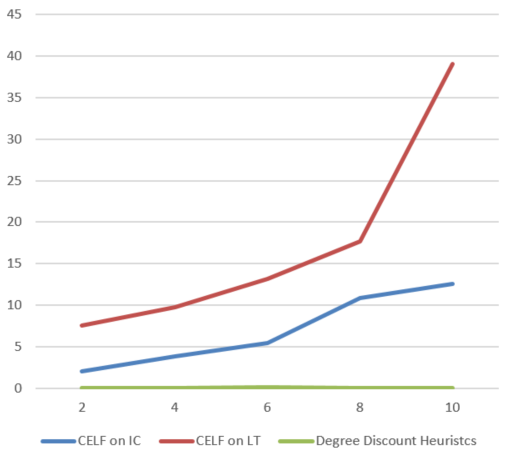
\includegraphics[width=\columnwidth]{result-time.png}}
\caption{Time difference}
\label{fig:result}
\end{figure}

\begin{figure}[!t]
\centerline{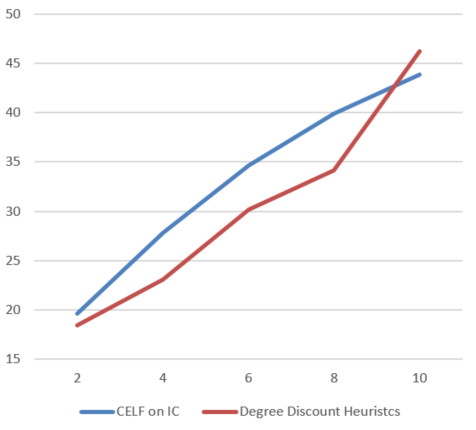
\includegraphics[width=\columnwidth]{ic-spread.png}}
\caption{Greedy V.S. heristics on IC model}
\label{fig:icdiff}
\end{figure}

\begin{figure}[!t]
\centerline{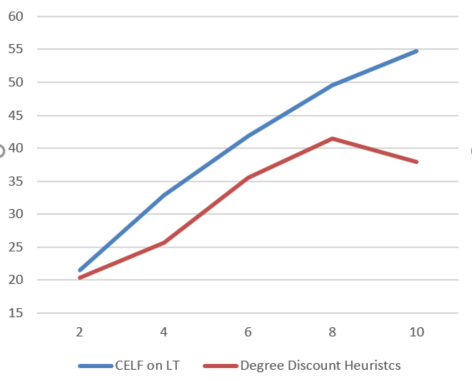
\includegraphics[width=\columnwidth]{lt-spread.png}}
\caption{Greedy V.S. heristics on LT model}
\label{fig:ltdiff}
\end{figure}

\section{Result Analysis and Further Direction}
As we can see from the results, the CELF improved greedy algorithm shows a better performance over heristics algorithm. However, the heuristic algorithm only take a very little time compared to time consumed by the greedy algorithms. Aslo, it is noticed that LT-based model takes longer time than IC-based model to evaluate.
\par
Note that the time of first iteration in CELF is the most time-consuming iteration, because all the vertices in the graph needs to be estimated. Thus, we may give some good heuristic algorithm for better performance during this phase. 
\par 
Also, the heuristic algorithm gives a results with small difference to that of greedy algorithm but with a large amount of time reduced. It may be a good way to find a better heuristc algorithm for better spread.
\section{Conclusion}

In this project, we almost implemented the art-of-state algorithms for the influence maximization problem. We get to know that different algorithms may be good at different aspects. We should be conscious when choosing the algorithm and take into the consideration of the computation tolerance.
 

\bibliographystyle{ieeetran}
\bibliography{reference}

\end{document}
